\pagebreak

Block name: Ramp\_ADC

Number of inputs: 1

Number of outputs: 0

Parameter list: NA

Block description: 
Single slope Analog to digital Converter. The input is to a FG comparator, which allows for higher dynamic range. The input current to the integrator is via a FG transistor and is set to 8nA.
Advanced users could change this from inside the block defination to change number of bits and speed of the ADC. The counter is implemented on the processor on-chip. Take DATA button is used to get the output of the Ramp ADC.
The output is stored in a .csv file called Results.csv. One can use the command Out=csvRead('Results.csv') to store it in a variable inside scilab. RAMP ADC performs data acquisition with a fixed sampling rate depending on the input voltage (100us maximum time between samples).
Hence the sampling rate of the system will be determined by the sampling rate of the DAC (ARB GEN block). 

\begin{figure}[H]  % jpg, png, or pdf
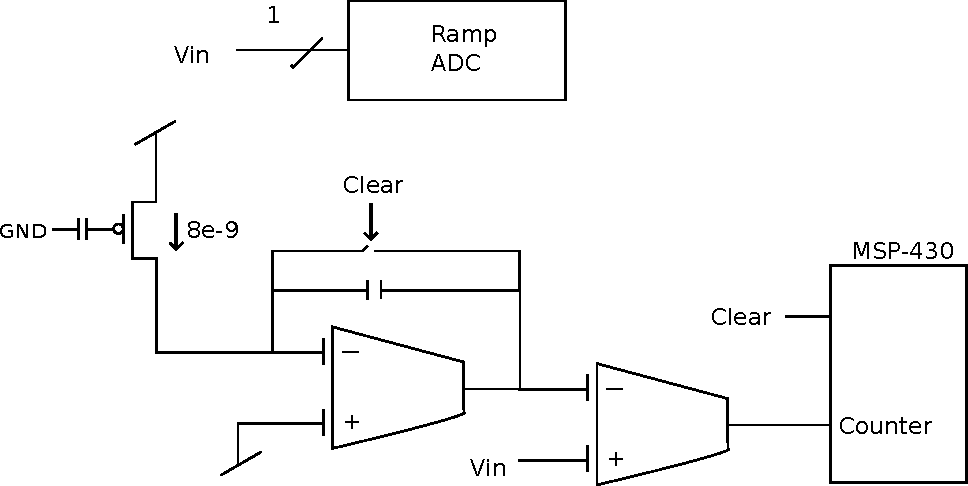
\includegraphics[width=300pt]{/home/ubuntu/rasp30/sci2blif/documentation/blocks_latex/figures/Ramp_ADC.pdf}
\end{figure}

